% Generated by aaai27/figures/scripts/make_tikz.py from figures/data/prelim_long256k.csv.
% Do not edit by hand; edit the data or the script and regenerate.
\begin{figure}[t]
\centering
\definecolor{vizblue}{HTML}{2A78D6}
\definecolor{vizorange}{HTML}{EB6834}
\definecolor{vizaqua}{HTML}{1BAF7A}
\definecolor{vizyellow}{HTML}{EDA100}
\definecolor{vizgrey}{HTML}{A9B0BB}
\definecolor{vizink}{HTML}{2B2F36}
\definecolor{vizink2}{HTML}{5F6570}
\definecolor{vizgrid}{HTML}{D9DCE1}
\resizebox{\linewidth}{!}{%
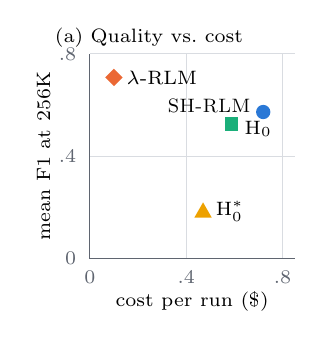
\begin{tikzpicture}[font=\scriptsize]
\draw[vizgrid, line width=0.3pt] (0,0.000) -- (2.600,0.000);
\draw[vizgrid, line width=0.3pt] (0.000,0) -- (0.000,2.600);
\node[anchor=east, text=vizink2] at (-0.05,0.000) {0};
\node[anchor=north, text=vizink2] at (0.000,-0.03) {0};
\draw[vizgrid, line width=0.3pt] (0,1.300) -- (2.600,1.300);
\draw[vizgrid, line width=0.3pt] (1.224,0) -- (1.224,2.600);
\node[anchor=east, text=vizink2] at (-0.05,1.300) {.4};
\node[anchor=north, text=vizink2] at (1.224,-0.03) {.4};
\draw[vizgrid, line width=0.3pt] (0,2.600) -- (2.600,2.600);
\draw[vizgrid, line width=0.3pt] (2.447,0) -- (2.447,2.600);
\node[anchor=east, text=vizink2] at (-0.05,2.600) {.8};
\node[anchor=north, text=vizink2] at (2.447,-0.03) {.8};
\draw[vizink2, line width=0.4pt] (0,0) -- (2.600,0) (0,0) -- (0,2.600);
\path[draw=vizaqua, fill=vizaqua, line width=0.6pt] (1.733,1.637) rectangle (1.877,1.782);
\node[anchor=west, inner sep=1pt] at (1.925,1.649) {$\mathrm{H}_0$};
\path[draw=vizyellow, fill=vizyellow, line width=0.6pt] (1.438,0.693) -- (1.346,0.532) -- (1.530,0.532) -- cycle;
\node[anchor=west, inner sep=1pt] at (1.558,0.601) {$\mathrm{H}_0^{*}$};
\path[draw=vizorange, fill=vizorange, line width=0.6pt] (0.306,2.397) -- (0.402,2.301) -- (0.306,2.205) -- (0.210,2.301) -- cycle;
\node[anchor=west, inner sep=1pt] at (0.426,2.301) {$\lambda$-RLM};
\path[draw=vizblue, fill=vizblue, line width=0.6pt] (2.202,1.862) circle (0.080);
\node[anchor=east, inner sep=1pt] at (2.082,1.942) {\textsc{SH-RLM}};
\node[rotate=90, anchor=south] at (-0.38,1.300) {mean F1 at 256K};
\node[anchor=north] at (1.300,-0.3) {cost per run (\$)};
\node[anchor=south west, inner sep=0pt] at (-0.45,2.680) {(a) Quality vs.\ cost};
\end{tikzpicture}
\hspace{0.4cm}
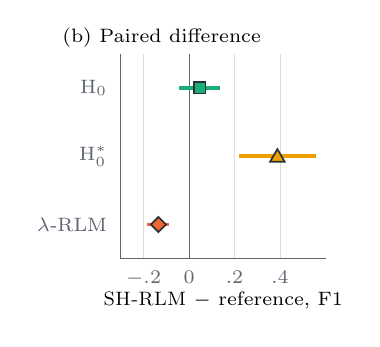
\begin{tikzpicture}[font=\scriptsize]
\draw[vizgrid, line width=0.3pt] (0.289,0) -- (0.289,2.600);
\node[anchor=north, text=vizink2] at (0.289,-0.03) {$-.2$};
\draw[vizgrid, line width=0.3pt] (0.867,0) -- (0.867,2.600);
\node[anchor=north, text=vizink2] at (0.867,-0.03) {0};
\draw[vizgrid, line width=0.3pt] (1.444,0) -- (1.444,2.600);
\node[anchor=north, text=vizink2] at (1.444,-0.03) {.2};
\draw[vizgrid, line width=0.3pt] (2.022,0) -- (2.022,2.600);
\node[anchor=north, text=vizink2] at (2.022,-0.03) {.4};
\draw[vizink2, line width=0.4pt] (0.867,0) -- (0.867,2.600);
\draw[vizink2, line width=0.4pt] (0,0) -- (2.600,0) (0,0) -- (0,2.600);
\draw[vizaqua, line width=1.4pt] (0.737,2.167) -- (1.254,2.167);
\path[draw=vizink, fill=vizaqua, line width=0.6pt] (0.933,2.095) rectangle (1.077,2.239);
\node[anchor=east, text=vizink2] at (-0.05,2.167) {$\mathrm{H}_0$};
\draw[vizyellow, line width=1.4pt] (1.502,1.300) -- (2.473,1.300);
\path[draw=vizink, fill=vizyellow, line width=0.6pt] (1.988,1.392) -- (1.896,1.231) -- (2.080,1.231) -- cycle;
\node[anchor=east, text=vizink2] at (-0.05,1.300) {$\mathrm{H}_0^{*}$};
\draw[vizorange, line width=1.4pt] (0.326,0.433) -- (0.612,0.433);
\path[draw=vizink, fill=vizorange, line width=0.6pt] (0.477,0.529) -- (0.573,0.433) -- (0.477,0.337) -- (0.381,0.433) -- cycle;
\node[anchor=east, text=vizink2] at (-0.05,0.433) {$\lambda$-RLM};
\node[anchor=north] at (1.300,-0.3) {\textsc{SH-RLM} $-$ reference, F1};
\node[anchor=south west, inner sep=0pt] at (-0.75,2.680) {(b) Paired difference};
\end{tikzpicture}
}
\caption{256K OOLONG-Pairs test (DeepSeek-V3.2; 9 tasks $\times$ 3
attempts per condition). (a)~Mean F1 against mean cost per run.
(b)~\shrlm minus each reference with task-level paired bootstrap 95\%
intervals; right of 0 favors \shrlm. Data as in \Cref{tab:long}.}
\label{fig:long}
\end{figure}
